\documentclass{article}

\title{Latent Variable Model and Data Generation}
\author{}
\date{}

\usepackage{amsmath}
\usepackage{bm}
\usepackage{Sweave}
\usepackage{graphicx}
\begin{document}
\Sconcordance{concordance:multivarExt2.tex:multivarExt2.Rnw:1 42 1 1 3 2 0 1 3 1 0 4 %
1 1 3 1 0 2 1 1 3 1 0 3 1 1 3 1 0 1 16 14 0 1 8 6 0 1 3 1 0 1 1 3 0 1 2 %
67 1 1 48 50 0 1 2 1 3 5 0 1 2 2 1 1 17 16 0 1 3 1 0 1 3 4 0 1 2 24 1 1 %
3 2 0 1 1 1 5 3 0 1 3 1 0 1 1 1 6 5 0 1 7 5 0 1 6 4 0 1 3 1 0 1 3 2 0 1 %
1 1 2 1 3 2 0 1 1 1 3 1 0 4 1 1 3 1 0 1 1 1 6 5 0 1 1 1 3 1 0 1 3 1 0 1 %
3 1 0 1 1 1 3 1 0 1 3 1 0 1 3 1 0 3 1 1 3 1 0 1 1 1 3 1 0 1 8 7 0 1 1 3 %
0 1 2 37 1}


\maketitle

\section{Introduction}

This document describes the theoretical framework for a latent variable model used to generate data and estimate model parameters using Bayesian inference. The model is implemented in Stan and involves the generation of latent variables and observed data using a Vector Autoregressive (VAR) process.

\section{Data Generation}

We generate data for $N_{\text{people}} = 10$ individuals over $N_{\text{timepoints}} = 50$ time points, with an initial burn-in period of $N_{\text{burnins}} = 25$ time points. The latent variables are generated using a VAR(1) model, and the observed data is generated by adding noise to the latent variables.

\subsection{VAR(1) Model}
The latent variables $\bm{F}_t = [F_{t1}, F_{t2}]^\top$ are generated using the following VAR(1) process:
\[
\bm{F}_t = \bm{\Phi} \bm{F}_{t-1} + \bm{\epsilon}_t, \quad \bm{\epsilon}_t \sim \mathcal{N}(\bm{0}, \bm{I}),
\]
where $\bm{\Phi}$ is the coefficient matrix:
\[
\bm{\Phi} = \begin{bmatrix} 0.5 & 0.2 \\ -0.3 & 0.4 \end{bmatrix}.
\]

\subsection{Observed Data}
The observed data $\bm{Y}_1$ and $\bm{Y}_2$ are generated by adding Gaussian noise to the latent variables:
\[
Y_{1tij} = F_{ti1} + \eta_{1tij}, \quad \eta_{1tij} \sim \mathcal{N}(0, 0.1),
\]
\[
Y_{2tij} = F_{ti2} + \eta_{2tij}, \quad \eta_{2tij} \sim \mathcal{N}(0, 0.1),
\]
for $i = 1, \ldots, N_{\text{people}}$, $j = 1, 2, 3$, and $t = 1, \ldots, N_{\text{timepoints}}$.

\begin{Schunk}
\begin{Sinput}
> # Remove all objects
> rm(list = ls())
> # Load necessary libraries
> library(forecast)
> library(rstan)
> library(loo)
> library(ggplot2)
> library(bayesplot)
> # Define parameters for data generation
> n_people <- 10
> n_burnins <- 25
> n_timepoints <- 50
> # Data generation for the latent variable model
> set.seed(123)
> F <- array(0, dim = c(n_people, 2, n_timepoints + n_burnins))
> Y1 <- array(0, dim = c(n_people, 3, n_timepoints))
> Y2 <- array(0, dim = c(n_people, 3, n_timepoints))
> # Coefficients for VAR(1) model
> phi <- matrix(c(0.5, 0.2, -0.3, 0.4), nrow = 2, ncol = 2)
> for (i in 1:n_people) {
+   # Initial values for F
+   F[i, , 1:2] <- matrix(rnorm(4, 0, 1), nrow = 2) # Initialize the first two timepoints
+   
+   # Generate latent variables F using VAR(1) model
+   for (t in 3:(n_burnins + n_timepoints)) {
+     F[i, , t] <- phi %*% F[i, , t-1] + rnorm(2, 0, 0.1)
+   }
+   
+   # Generate observed data Y1 and Y2 from latent variables F
+   for (j in 1:3) {
+     Y1[i, j, ] <- F[i, 1, (n_burnins + 1):(n_burnins + n_timepoints)] + rnorm(n_timepoints, 0, 0.1)
+     Y2[i, j, ] <- F[i, 2, (n_burnins + 1):(n_burnins + n_timepoints)] + rnorm(n_timepoints, 0, 0.1)
+   }
+ }
> # Prepare data for Stan
> data_list <- list(
+   N_people = n_people,
+   N_timepoints = n_timepoints,
+   Y1 = Y1,
+   Y2 = Y2
+ )
> # Set Stan options
> options(mc.cores = parallel::detectCores())
> rstan_options(auto_write = TRUE)
\end{Sinput}
\end{Schunk}

\section{Stan Model}
The Stan model defines the prior distributions for the parameters, the likelihood of the data given the parameters, and the generated quantities for posterior predictive checks.

\subsection{Data Block}
The data block specifies the input data for the Stan model:
\begin{verbatim}
data {
  int<lower=1> N_people;
  int<lower=1> N_timepoints;
  matrix[3, N_timepoints] Y1[N_people];
  matrix[3, N_timepoints] Y2[N_people];
}
\end{verbatim}

\subsection{Parameters Block}
The parameters block defines the parameters to be estimated:
\begin{verbatim}
parameters {
  matrix[N_timepoints, 2] F[N_people]; // Latent variables F1 and F2
  cholesky_factor_corr[2] L;           // Cholesky decomposition of the covariance matrix
  real<lower=0> sigma[2, 3];           // Standard deviation of observation noise
  matrix[2, 2] A;                      // Coefficient matrix for VAR(1)
}
\end{verbatim}

\subsection{Model Block}
The model block defines the prior distributions and the likelihood:
\begin{verbatim}
model {
  L ~ lkj_corr_cholesky(2.0); // Prior distribution for the covariance matrix
  to_vector(A) ~ normal(0, 1); // Prior for VAR coefficients
  for (i in 1:N_people) {
    for (t in 2:N_timepoints) { // VAR(1) model
      F[i, t] ~ multi_normal_cholesky(A * F[i, t-1]', diag_matrix(rep_vector(1, 2)) * L);
    }
    F[i, 1] ~ multi_normal_cholesky(rep_vector(0, 2), diag_matrix(rep_vector(1, 2)) * L); // Initial state
    for (t in 1:N_timepoints) {
      for (k in 1:3) {
        Y1[i, k, t] ~ normal(F[i, t, 1], sigma[1, k]);
        Y2[i, k, t] ~ normal(F[i, t, 2], sigma[2, k]);
      }
    }
  }
}
\end{verbatim}

\subsection{Generated Quantities Block}
The generated quantities block calculates the log likelihood and posterior predictive distributions:
\begin{verbatim}
generated quantities {
  vector[N_timepoints] log_lik[N_people];
  matrix[3, N_timepoints] y_hat1[N_people];
  matrix[3, N_timepoints] y_hat2[N_people];
  for (i in 1:N_people) {
    for (t in 1:N_timepoints) {
      log_lik[i, t] = 0;
      for (k in 1:3) {
        y_hat1[i, k, t] = normal_rng(F[i, t, 1], sigma[1, k]);
        y_hat2[i, k, t] = normal_rng(F[i, t, 2], sigma[2, k]);
        log_lik[i, t] += normal_lpdf(Y1[i, k, t] | F[i, t, 1], sigma[1, k]) +
                         normal_lpdf(Y2[i, k, t] | F[i, t, 2], sigma[2, k]);
      }
    }
  }
}
\end{verbatim}

\begin{Schunk}
\begin{Sinput}
> # Stan code for latent variable model
> stan_code <- "
+ data {
+   int<lower=1> N_people;
+   int<lower=1> N_timepoints;
+   matrix[3, N_timepoints] Y1[N_people];
+   matrix[3, N_timepoints] Y2[N_people];
+ }
+ parameters {
+   matrix[N_timepoints, 2] F[N_people]; // Latent variables F1 and F2
+   cholesky_factor_corr[2] L;           // Cholesky decomposition of the covariance matrix
+   real<lower=0> sigma[2, 3];           // Standard deviation of observation noise
+   matrix[2, 2] A;                      // Coefficient matrix for VAR(1)
+ }
+ model {
+   L ~ lkj_corr_cholesky(2.0); // Prior distribution for the covariance matrix
+   to_vector(A) ~ normal(0, 1); // Prior for VAR coefficients
+   for (i in 1:N_people) {
+     for (t in 2:N_timepoints) { // VAR(1) model
+       F[i, t] ~ multi_normal_cholesky(A * F[i, t-1]', diag_matrix(rep_vector(1, 2)) * L);
+     }
+     F[i, 1] ~ multi_normal_cholesky(rep_vector(0, 2), diag_matrix(rep_vector(1, 2)) * L); // Initial state
+     for (t in 1:N_timepoints) {
+       for (k in 1:3) {
+         Y1[i, k, t] ~ normal(F[i, t, 1], sigma[1, k]);
+         Y2[i, k, t] ~ normal(F[i, t, 2], sigma[2, k]);
+       }
+     }
+   }
+ }
+ generated quantities {
+   vector[N_timepoints] log_lik[N_people];
+   matrix[3, N_timepoints] y_hat1[N_people];
+   matrix[3, N_timepoints] y_hat2[N_people];
+   for (i in 1:N_people) {
+     for (t in 1:N_timepoints) {
+       log_lik[i, t] = 0;
+       for (k in 1:3) {
+         y_hat1[i, k, t] = normal_rng(F[i, t, 1], sigma[1, k]);
+         y_hat2[i, k, t] = normal_rng(F[i, t, 2], sigma[2, k]);
+         log_lik[i, t] += normal_lpdf(Y1[i, k, t] | F[i, t, 1], sigma[1, k]) +
+                          normal_lpdf(Y2[i, k, t] | F[i, t, 2], sigma[2, k]);
+       }
+     }
+   }
+ }
+ "
\end{Sinput}
\end{Schunk}

\begin{Schunk}
\begin{Sinput}
> # Compile Stan model
> stan_model <- stan_model(model_code = stan_code)
\end{Sinput}
\end{Schunk}

\section{Model Fitting}

\begin{Schunk}
\begin{Sinput}
> # Set initial values based on data
> init_values <- function() {
+   F_init <- array(0, dim = c(n_people, n_timepoints, 2))
+   for (i in 1:n_people) {
+     for (t in 1:n_timepoints) {
+       F_init[i, t, 1] <- mean(data_list$Y1[i, , t])
+       F_init[i, t, 2] <- mean(data_list$Y2[i, , t])
+     }
+   }
+   list(
+     F = F_init,
+     L = diag(2),
+     sigma = matrix(runif(6, 0.1, 1), nrow = 2),
+     A = matrix(runif(4, -0.5, 0.5), nrow = 2)
+   )
+ }
> # Fit the model with better initial values
> fit <- sampling(stan_model, data = data_list, iter = 2000, chains = 4, init = init_values)
> # Extract samples
> samples <- extract(fit)
\end{Sinput}
\end{Schunk}

\section{Evaluation Metrics}
The model is evaluated using several metrics:

\subsection{Mean Squared Error (MSE)}
The MSE is calculated for each time point and each individual to measure the accuracy of the predicted values:
\[
\text{MSE} = \frac{1}{N} \sum_{i=1}^{N} (y_i - \hat{y}_i)^2
\]

\subsection{Log Likelihood}
The log likelihood is averaged over iterations to assess the model fit:
\[
\log L = \frac{1}{T} \sum_{t=1}^{T} \log p(\bm{y}_t | \bm{F}_t, \sigma)
\]

\subsection{Prediction Intervals}
95\% prediction intervals are calculated for the posterior predictive distribution to assess the model uncertainty:
\[
\hat{y}_{1, \text{lower}} = \text{quantile}(y_{\text{hat1}}, 0.025)
\]
\[
\hat{y}_{1, \text{upper}} = \text{quantile}(y_{\text{hat1}}, 0.975)
\]

\begin{Schunk}
\begin{Sinput}
> # Obtain the mean of the posterior predictive distribution
> y_hat1_mean <- apply(samples$y_hat1, c(2, 3, 4), mean) # Result is (n_people, 3, n_timepoints)
> y_hat2_mean <- apply(samples$y_hat2, c(2, 3, 4), mean) # Result is (n_people, 3, n_timepoints)
> # Define function to calculate MSE
> calculate_mse <- function(y_hat, y_true) {
+   return(mean((y_hat - y_true)^2))
+ }
> # Calculate MSE
> mse1 <- array(0, dim = c(n_people, n_timepoints))
> mse2 <- array(0, dim = c(n_people, n_timepoints))
> for (i in 1:n_people) {
+   for (t in 1:n_timepoints) {
+     mse1[i, t] <- calculate_mse(y_hat1_mean[i, , t], data_list$Y1[i, , t])
+     mse2[i, t] <- calculate_mse(y_hat2_mean[i, , t], data_list$Y2[i, , t])
+   }
+ }
> # Plot MSE
> mse_df1 <- data.frame(
+   Time = rep(1:n_timepoints, n_people),
+   MSE = as.vector(mse1),
+   Person = rep(1:n_people, each = n_timepoints)
+ )
> mse_df2 <- data.frame(
+   Time = rep(1:n_timepoints, n_people),
+   MSE = as.vector(mse2),
+   Person = rep(1:n_people, each = n_timepoints)
+ )
> # Save MSE plots
> pdf("mse_plot_y1.pdf")
> ggplot(mse_df1, aes(x = Time, y = MSE, color = as.factor(Person))) + 
+   geom_line() + 
+   labs(title = "MSE for Y1", x = "Time", y = "MSE", color = "Person")
> dev.off()
> pdf("mse_plot_y2.pdf")
> ggplot(mse_df2, aes(x = Time, y = MSE, color = as.factor(Person))) + 
+   geom_line() + 
+   labs(title = "MSE for Y2", x = "Time", y = "MSE", color = "Person")
> dev.off()
> # Plot posterior distributions of VAR coefficients and Cholesky factors
> posterior <- as.array(fit)
> pdf("posterior_distributions_VAR.pdf")
> mcmc_areas(posterior, pars = c("A[1,1]", "A[1,2]", "A[2,1]", "A[2,2]"))
> mcmc_areas(posterior, pars = c("L[1,1]", "L[2,2]", "L[1,2]", "L[2,1]"))
> dev.off()
> # Plot predicted vs observed values for the first person
> pdf("predicted_vs_observed_y1.pdf")
> person_index <- 1
> for (k in 1:3) {
+   plot(1:n_timepoints, data_list$Y1[person_index, k, ], type = "l", col = "blue", ylim = range(c(data_list$Y1[person_index, k, ], y_hat1_mean[person_index, k, ])), ylab = "Y1", xlab = "Time")
+   lines(1:n_timepoints, y_hat1_mean[person_index, k, ], col = "red")
+   title(paste("Observed vs Predicted Y1 for Person", person_index, "Variable", k))
+   legend("topright", legend = c("Observed", "Predicted"), col = c("blue", "red"), lty = 1)
+ }
> dev.off()
> # Extract log likelihood
> log_lik <- extract_log_lik(fit)
> # Check the structure of log_lik
> str(log_lik)  # Should show a matrix with dimensions (iterations, 10 * 50)
> # Reshape log_lik to (iterations, n_people, n_timepoints)
> iterations <- dim(log_lik)[1]
> log_lik_reshaped <- array(log_lik, dim = c(iterations, n_people, n_timepoints))
> # Average log likelihood over iterations
> log_lik_mean <- apply(log_lik_reshaped, c(2, 3), mean)  # Average over iterations, keeping (n_people, n_timepoints)
> # Optionally, average over people to get a single time series
> log_lik_mean_over_people <- apply(log_lik_mean, 2, mean)
> # Plot log likelihood over time
> pdf("log_likelihood_over_time.pdf")
> plot(1:n_timepoints, log_lik_mean_over_people, type = "l", col = "black", ylab = "Log Likelihood", xlab = "Time")
> title("Log Likelihood over Time")
> dev.off()
> # Calculate 95% prediction intervals
> y_hat1_lower <- apply(samples$y_hat1, c(2, 3, 4), quantile, probs = 0.025)
> y_hat1_upper <- apply(samples$y_hat1, c(2, 3, 4), quantile, probs = 0.975)
> # Plot prediction intervals vs observed values for the first person
> pdf("prediction_intervals_y1.pdf")
> for (k in 1:3) {
+   plot(1:n_timepoints, data_list$Y1[person_index, k, ], type = "l", col = "blue", ylim = range(c(data_list$Y1[person_index, k, ], y_hat1_lower[person_index, k, ], y_hat1_upper[person_index, k, ])), ylab = "Y1", xlab = "Time")
+   lines(1:n_timepoints, y_hat1_mean[person_index, k, ], col = "red")
+   lines(1:n_timepoints, y_hat1_lower[person_index, k, ], col = "grey", lty = 2)
+   lines(1:n_timepoints, y_hat1_upper[person_index, k, ], col = "grey", lty = 2)
+   title(paste("Observed vs Predicted Y1 with Prediction Interval for Person", person_index, "Variable", k))
+   legend("topright", legend = c("Observed", "Predicted", "95% Interval"), col = c("blue", "red", "grey"), lty = c(1, 1, 2))
+ }
> dev.off()
\end{Sinput}
\end{Schunk}

\begin{figure}[h]
  \centering
  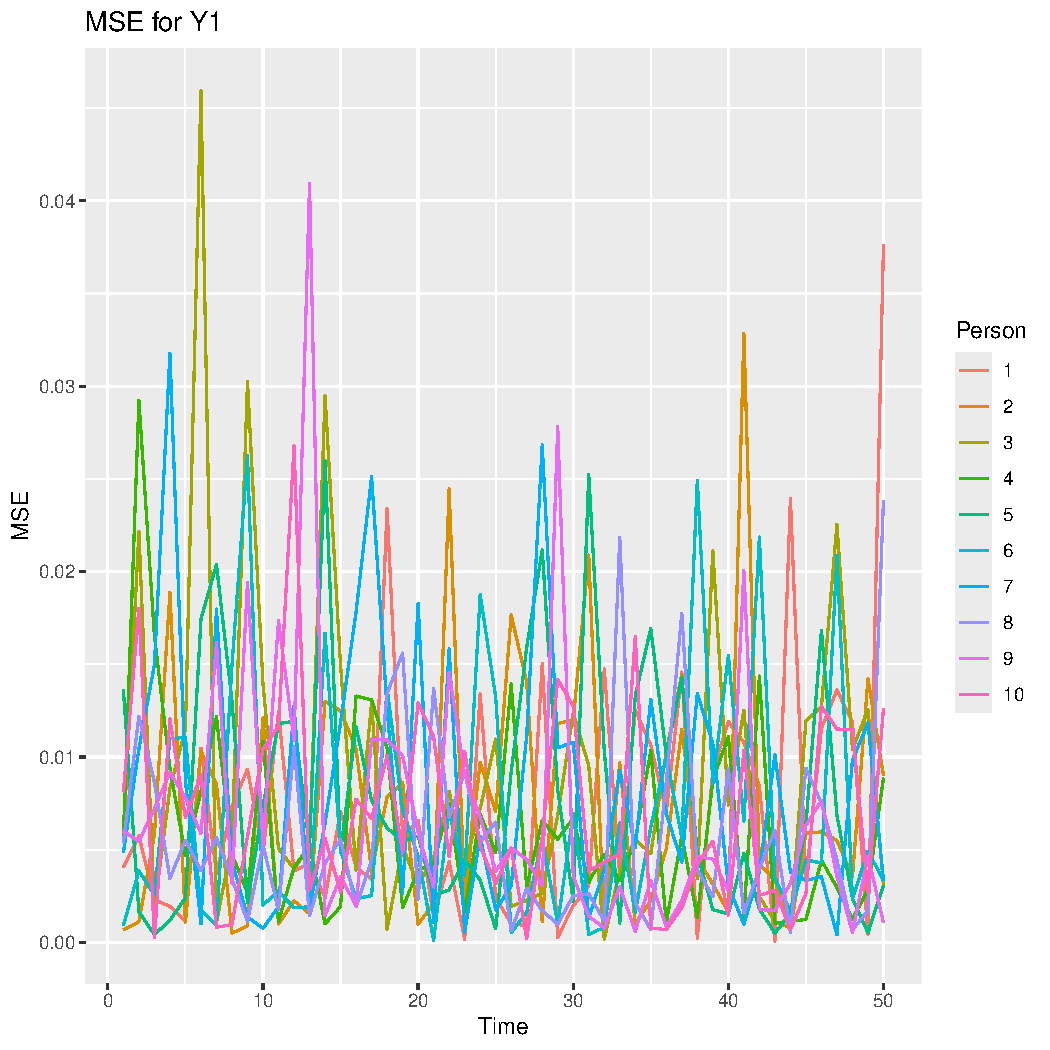
\includegraphics[width=\textwidth]{mse_plot_y1.pdf}
  \caption{MSE for Y1}
\end{figure}

\begin{figure}[h]
  \centering
  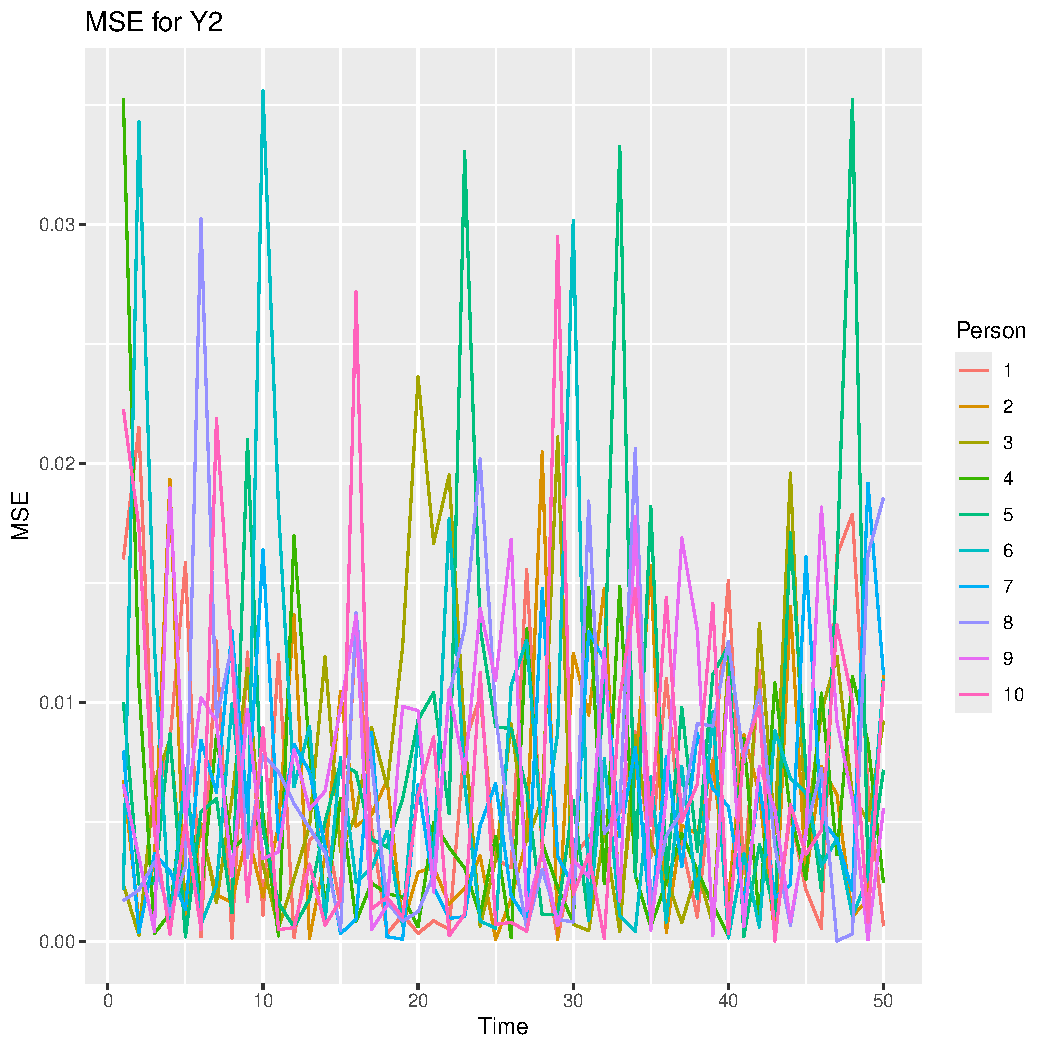
\includegraphics[width=\textwidth]{mse_plot_y2.pdf}
  \caption{MSE for Y2}
\end{figure}

\begin{figure}[h]
  \centering
  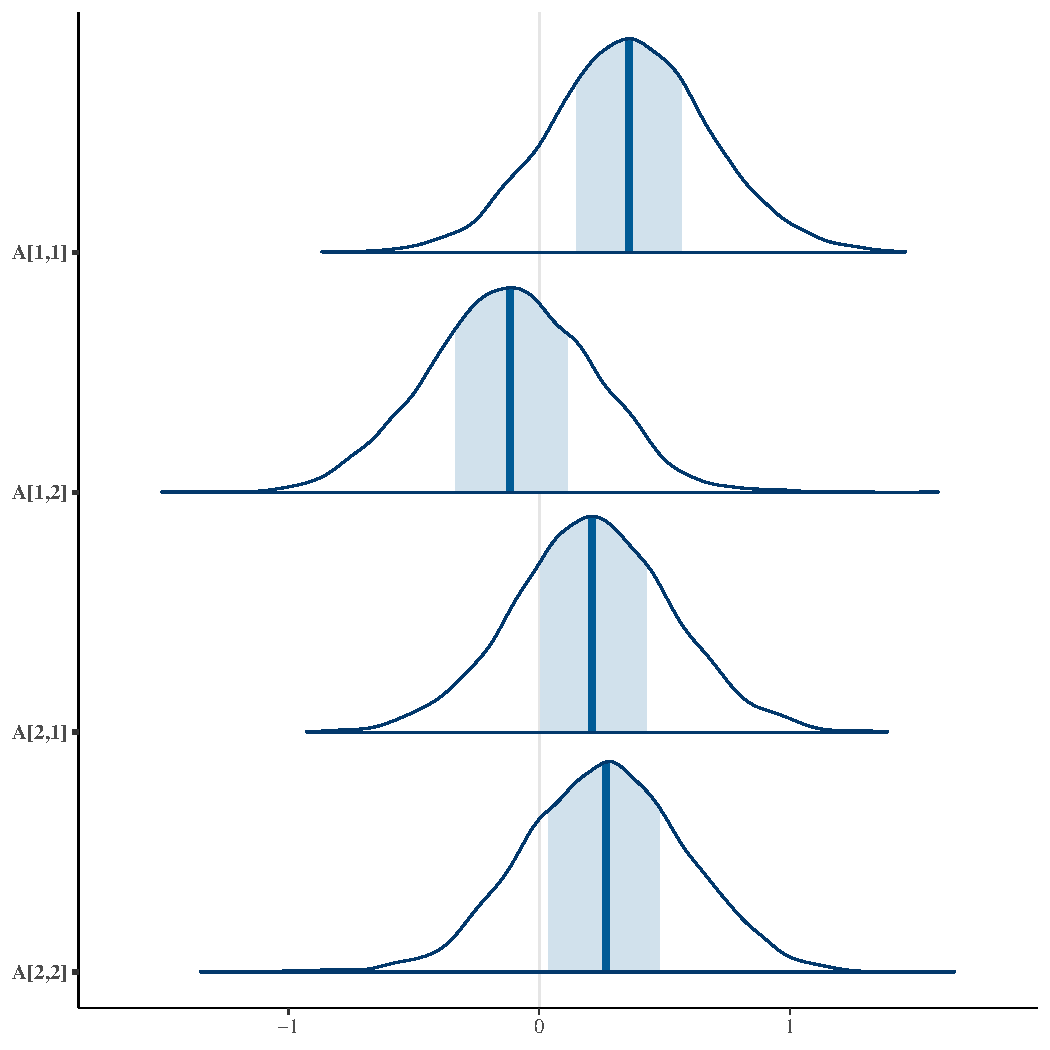
\includegraphics[width=\textwidth]{posterior_distributions_VAR.pdf}
  \caption{Posterior Distributions of VAR Coefficients and Cholesky Factors}
\end{figure}

\begin{figure}[h]
  \centering
  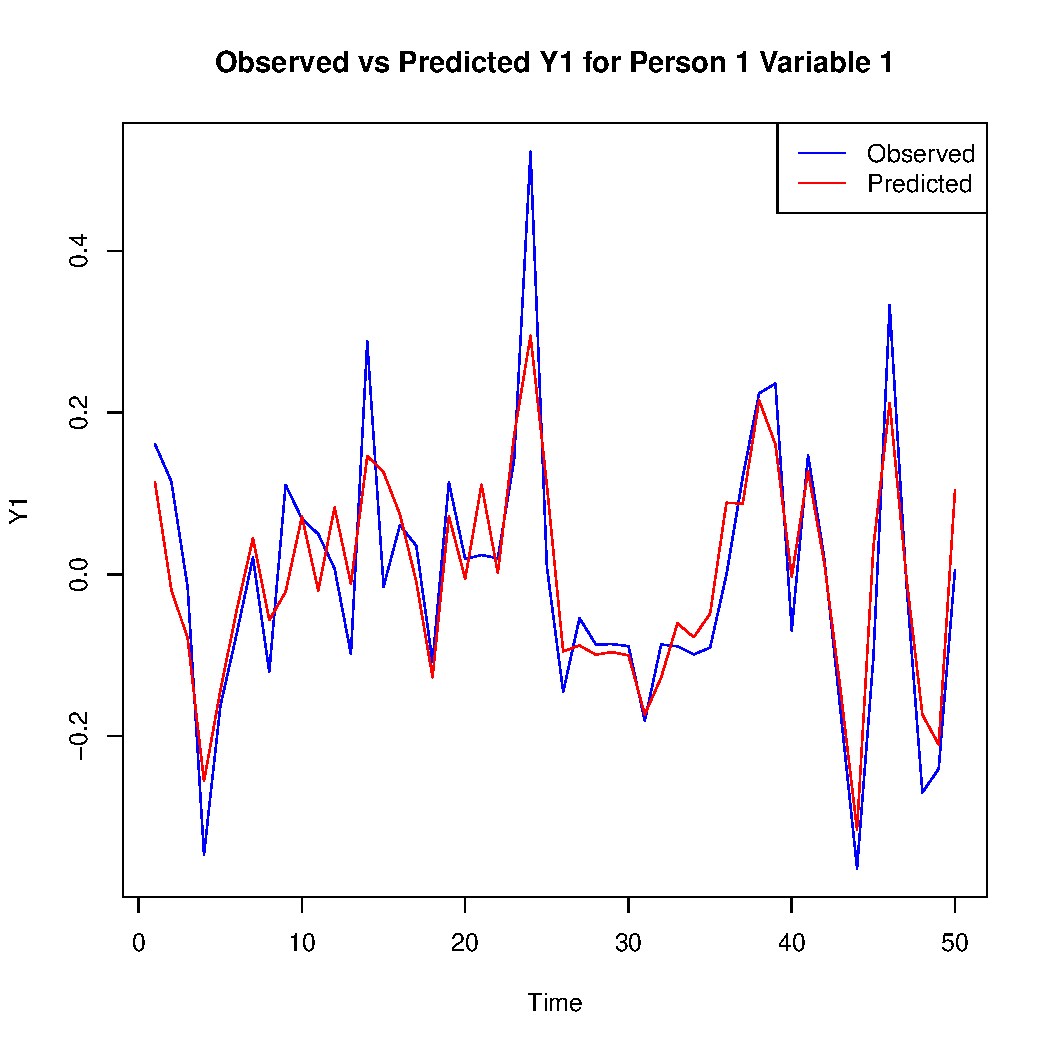
\includegraphics[width=\textwidth]{predicted_vs_observed_y1.pdf}
  \caption{Observed vs Predicted Y1 for Person 1}
\end{figure}

\begin{figure}[h]
  \centering
  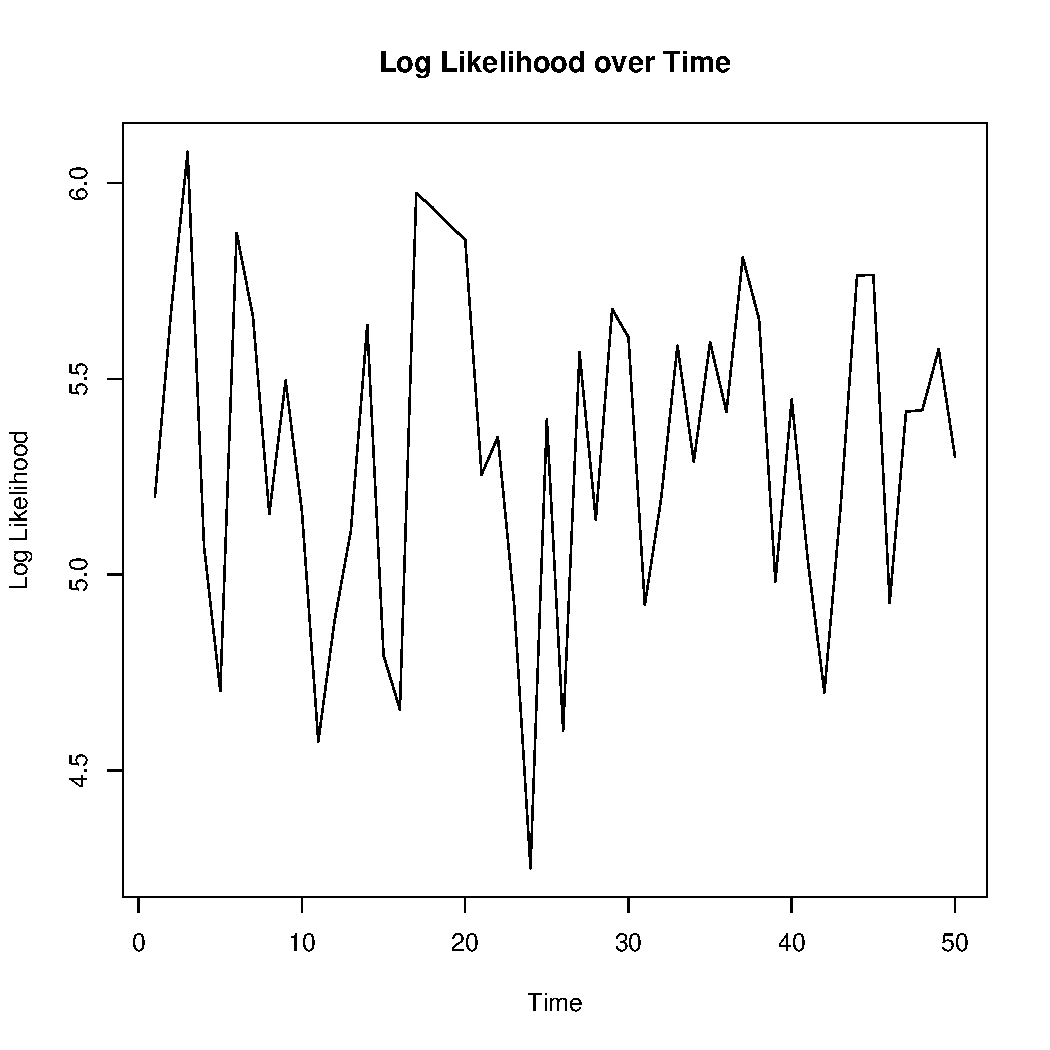
\includegraphics[width=\textwidth]{log_likelihood_over_time.pdf}
  \caption{Log Likelihood over Time}
\end{figure}

\begin{figure}[h]
  \centering
  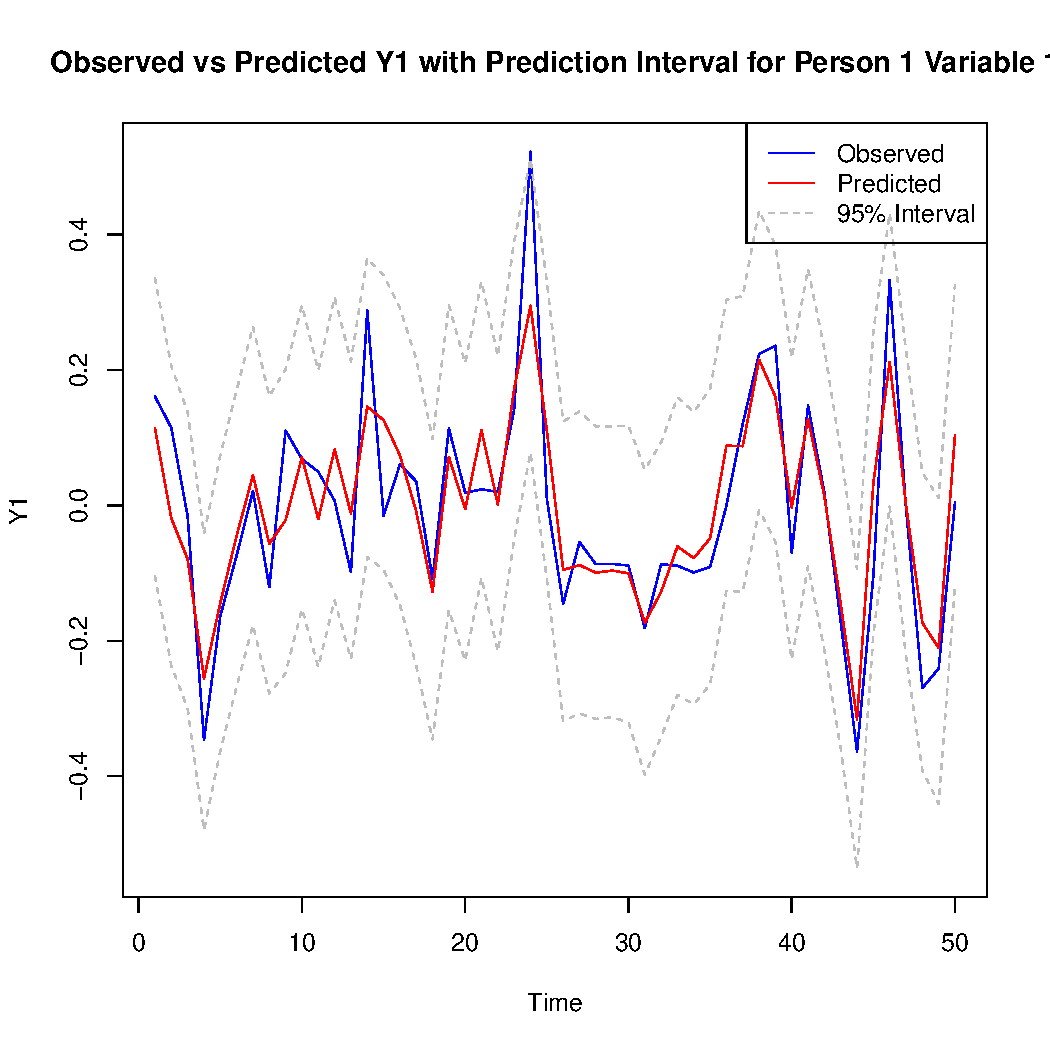
\includegraphics[width=\textwidth]{prediction_intervals_y1.pdf}
  \caption{Observed vs Predicted Y1 with Prediction Interval for Person 1}
\end{figure}

\end{document}
